\documentclass{article}

\usepackage{fancyhdr} % Required for custom headers
\usepackage{lastpage} % Required to determine the last page for the footer
\usepackage{extramarks} % Required for headers and footers
\usepackage{graphicx} % Required to insert images
\usepackage{lipsum} % Used for inserting dummy 'Lorem ipsum' text into the template
\usepackage[utf8]{inputenc}
\usepackage{enumerate}
\usepackage{amsmath}
\usepackage{wrapfig}

% Margins
\topmargin=-0.45in
\evensidemargin=0in
\oddsidemargin=0in
\textwidth=6.5in
\textheight=9.0in
\headsep=0.25in 

\linespread{1.1} % Line spacing

% Set up the header and footer
\pagestyle{fancy}
\lhead{\hmwkAuthorName} % Top left header
\chead{\hmwkClass\ \hmwkTitle} % Top center header
\rhead{\firstxmark} % Top right header
\lfoot{\lastxmark} % Bottom left footer
\cfoot{} % Bottom center footer
\rfoot{Page\ \thepage\ of\ \pageref{LastPage}} % Bottom right footer
\renewcommand\headrulewidth{0.4pt} % Size of the header rule
\renewcommand\footrulewidth{0.4pt} % Size of the footer rule

\setlength\parindent{0pt} % Removes all indentation from paragraphs

%----------------------------------------------------------------------------------------
%	DOCUMENT STRUCTURE COMMANDS
%	Skip this unless you know what you're doing
%----------------------------------------------------------------------------------------

% Header and footer for when a page split occurs within a problem environment
\newcommand{\enterProblemHeader}[1]{
\nobreak\extramarks{#1}{#1 continued on next page\ldots}\nobreak
\nobreak\extramarks{#1 (continued)}{#1 continued on next page\ldots}\nobreak
}

% Header and footer for when a page split occurs between problem environments
\newcommand{\exitProblemHeader}[1]{
\nobreak\extramarks{#1 (continued)}{#1 continued on next page\ldots}\nobreak
\nobreak\extramarks{#1}{}\nobreak
}

\setcounter{secnumdepth}{0} % Removes default section numbers
\newcounter{homeworkProblemCounter} % Creates a counter to keep track of the number of problems

\newcommand{\homeworkProblemName}{}
\newenvironment{homeworkProblem}[1][Problem \arabic{homeworkProblemCounter}]{ % Makes a new environment called homeworkProblem which takes 1 argument (custom name) but the default is "Problem #"
\stepcounter{homeworkProblemCounter} % Increase counter for number of problems
\renewcommand{\homeworkProblemName}{#1} % Assign \homeworkProblemName the name of the problem
\section{\homeworkProblemName} % Make a section in the document with the custom problem count
\enterProblemHeader{\homeworkProblemName} % Header and footer within the environment
}{
\exitProblemHeader{\homeworkProblemName} % Header and footer after the environment
}

\newcommand{\problemAnswer}[1]{ % Defines the problem answer command with the content as the only argument
\noindent\framebox[\columnwidth][c]{\begin{minipage}{0.98\columnwidth}#1\end{minipage}} % Makes the box around the problem answer and puts the content inside
}

\newcommand{\homeworkSectionName}{}
\newenvironment{homeworkSection}[1]{ % New environment for sections within homework problems, takes 1 argument - the name of the section
\renewcommand{\homeworkSectionName}{#1} % Assign \homeworkSectionName to the name of the section from the environment argument
\subsection{\homeworkSectionName} % Make a subsection with the custom name of the subsection
\enterProblemHeader{\homeworkProblemName\ [\homeworkSectionName]} % Header and footer within the environment
}{
\enterProblemHeader{\homeworkProblemName} % Header and footer after the environment
}

%----------------------------------------------------------------------------------------
%	NAME AND CLASS SECTION
%----------------------------------------------------------------------------------------

\newcommand{\hmwkTitle}{} % Assignment title
\newcommand{\subt}{} % Assignment title
%\newcommand{\hmwkDueDate}{Canale D: 18 giugno 2015} % Due date
\newcommand{\hmwkClass}{Laboratorio di Meccanica - canale B (Cl-Git) - A.A. 2025-2026 - Proff. S. De Cecco, L. Cunqueiro Mendez} % Course/class
\newcommand{\hmwkClassTime}{} % Class/lecture time
\newcommand{\hmwkClassInstructor}{} % Teacher/lecturer
\newcommand{\hmwkAuthorName}{} % Your name


%----------------------------------------------------------------------------------------
%	PHANTOM TEXT
%----------------------------------------------------------------------------------------

\newcommand{\spazio}[1]{\phantom{#1}}

%----------------------------------------------------------------------------------------
%	TITLE PAGE
%----------------------------------------------------------------------------------------

\title{
\vspace{2in}
\textmd{\textbf{\hmwkClass\ \hmwkTitle}}\\
\vspace{0.3in}
\Large{\textbf{\subt}}\\
\normalsize\vspace{0.1in}\small{\hmwkDueDate}\\
\vspace{0.1in}\large{\textit{\hmwkClassInstructor\ \hmwkClassTime}}
\vspace{3in}
}

\author{\textbf{\hmwkAuthorName}}
\date{} % Insert date here if you want it to appear below your name

%----------------------------------------------------------------------------------------


\begin{document}

%{\Large {\bf \underline{Prova pratica individuale - 12/06/2017}}}\flushleft
\center{\center \Large {\bf \underline{Seconda Prova Pratica Individuale - 9 giugno 2026}}}\flushleft
\vspace{0.1in}
{\Large Cognome: Ferretti Nome: Liam Matricola: 2252865}
\vspace{0.1in}

\small Formato nome file relazione ({\bf MAX 7 PAG.}) da caricare: {\bf BX-YY\_COGNOME\_NOME\_PPI2-2026.pdf}

\section{Strumenti di misura}

Nella Tabella \ref{tab:infoStrumeni} sono riassunte le caratteristiche degli strumenti impiegati per la conduzione dell'esperimento. 

Per tutti gli strumenti usati, dopo aver verificato l'eventuale presenza di offset, è stata calcolata l'incertezza di tipo B, tramite la seguente formula:
\begin{equation}
	\sigma_b = \frac{\text{risoluzione}}{\sqrt{12}}
	\label{eq:sigma_b}
\end{equation}
Negli strumenti non vi sono offset in quanto, nel caso della bilancia e del cronometro digitale vi è la possibilità di tarare/azzerare lo strumento prima di ogni misura, nel caso del nonio invece, a becchi chiusi, restituisce il valore aspettato 0.

{\def\arraystretch{2}\tabcolsep=12pt
\begin{table}[h!]
	\begin{center}
		\begin{tabular}{|l|ccccc|c}
			\hline
			strumento  & portata & risoluzione & $\sigma_B$ & offset & unit\`a \\
			\hline 
			Calibro a nonio & 15.000  & 0.050 & 0.014 & -- & mm  \\
			\hline
			Bilancia & 2000.000 & 0.100 & 0.029 & -- & g  \\
			\hline
			Cronometro digitale & Virt. Infinita  & 0.0100 & 0.0029& -- & s  \\
			\hline
		\end{tabular}
	\end{center}
	\caption{Caratteristiche degli strumenti usati.}
	\label{tab:infoStrumeni}
\end{table}
}

\newpage


\newpage
\section{Parte 1: descrizione delle misure, analisi dati (con le formule utilizzate) e risultati}
\subsection{Determinazione di $R$}

La determinazione della distanza $R$ dal centro di rotazione del disco al centro dei fori è stata eseguita tramite una misura indiretta. Non essendo possibile individuare e misurare direttamente il centro e il centro dei fori, si è scelto di scomporre la distanza nella somma di tre contributi distinti, ciascuno misurato ripetutamente (5 volte) per ridurne l'incertezza:
\begin{enumerate}
    \item Il diametro del perno centrale del disco ($D_p$).
    \item La distanza tra il bordo esterno del perno centrale e il bordo interno del foro del bullone ($d_f$).
    \item Il diametro del foro di alloggiamento del bullone ($D_b$).
\end{enumerate}

La stima della distanza finale $R$ è data quindi dalla relazione geometrica:
\begin{equation}
    R = \frac{D_p}{2} + d_f + \frac{D_b}{2}
    \label{eq:calcoloR}
\end{equation}

Per ciascuna delle tre grandezze, l'incertezza totale ($\sigma_{tot}$) è stata ricavata tramite la formula \ref{eq:sigma_tot}, usando l'incertezza statistica di tipo A derivata dalla formula \ref{eq:varianzaCampionaria} e l'incertezza di tipo B presente in tabella \ref{tab:infoStrumeni}

\begin{equation}
    \sigma_{n - 1} = \sqrt{\frac{\sum_i (x_i - \bar{x})^2}{n - 1}}
    \label{eq:varianzaCampionaria}
\end{equation}

\begin{equation}
	\sigma_{tot} = \sqrt{\sigma_a^2 + \sigma_b^2}
	\label{eq:sigma_tot}
\end{equation}

Assumendo l'indipendenza e la non-correlazione tra le tre diverse operazioni di misura, l'incertezza finale su $R$ ($\sigma_R$) è stata ricavata tramite la formula \ref{eq:calcoloR}:
\begin{equation}
    \sigma_R = \sqrt{\left(\frac{1}{2}\sigma_{D_p}\right)^2 + \sigma_{d_f}^2 + \left(\frac{1}{2}\sigma_{D_b}\right)^2}
\end{equation}

Per la disposizione dei bulloni, al fine di garantire che la risultante del momento della forza peso rispetto al baricentro rimanesse nulla (evitando l'introduzione di sbilanciamenti), i bulloni sono stati posti in posizione diametralmente opposta, tranne nel caso $n = 3$ che sono stati disposti sui veritici di un triangolo equilatero.

\subsection{Determinazione di $T$}
Per ogni configurazione sono state effettuate 5 misure di 5 periodi completi, tramite le quali è stato possibile stimare l'incertezza di tipo A, tramite la varianza campionaria formula \ref{eq:varianzaCampionaria}.
L'incertezza totale sul tempo di 5 oscillazioni è stata ottenuta sommando in quadratura l'incertezza statistica di tipo A e l'incertezza di risoluzione del cronometro (formula~\ref{eq:sigma_tot}), quindi per trovare il periodo best di ogni configurazione è stata usata la formula \ref{eq:formulaPeriodi}:

\begin{equation}
    \hat{T}_i = \frac{\hat{t}_{best_i}}{5}
    \label{eq:formulaPeriodi}
\end{equation}

L'incertezza sul singolo periodo $T$ e sul suo quadrato $T^2$ è stata propagata come:
\begin{equation}
    \sigma_T = \frac{\sigma_{t_5}}{5}, \qquad \sigma_{T^2} = 2\,T\,\sigma_T
    \label{eq:incT}
\end{equation}

\subsection{Determinazione di $M_B$}
La massa totale $M_B$ per le diverse configurazioni è stata determinata a partire dalla pesata individuale dei $N=6$ bulloni disponibili. L'analisi statistica del campione fornisce una massa media:
\begin{equation}
    \bar{M} = 53.600 \pm 0.039 \text{ g}
\end{equation}
la cui incertezza $\sigma_{M_{bullone}}$ deriva dalla formula \ref{eq:sigma_tot}, nella quale $\sigma_a$ equivale alla varianza campionaria stimata tramite la formula \ref{eq:varianzaCampionaria} e la $\sigma_b$ tramite la formula \ref{eq:sigma_b}.

L'incertezza totale in funzione del numero di bulloni è stata calcolata tramite:
\begin{equation}
    \sigma_{M_B} = \sqrt{n} \cdot \sigma_{M_{bullone}}
\end{equation}

\newpage

{\def\arraystretch{2}\tabcolsep=12pt
	\begin{table}[h!]
		\begin{center}
			\begin{tabular}{|c|}
				\hline
				$R $ \\
				\hline  
				$116.363 \pm 0.087$ mm \\
				\hline
			\end{tabular}
		\end{center}
		\caption{Misura della distanza richiesta nella domanda 1)}
		\label{tab2}
	\end{table}
}

{\def\arraystretch{2}\tabcolsep=12pt
	\begin{table}[h!]
		\begin{center}
			\begin{tabular}{|l|c|c|c|}
				\hline
				n. di bulloni inseriti & $M_B$ & $T$ &  $T^2$  \\
				\hline
				0 & --                    & $6.7460 \pm 0.0032$ s & $45.509 \pm 0.043\ \mathrm{s}^2$\\
				\hline
				2 & $107.600 \pm 0.055$ g & $8.3316 \pm 0.0042$ s & $69.416 \pm 0.069\ \mathrm{s}^2$ \\
				\hline
				3 & $160.800 \pm 0.068$ g & $8.9792 \pm 0.0027$ s & $80.626 \pm 0.049\ \mathrm{s}^2$ \\
				\hline
				4 & $214.400 \pm 0.078$ g & $9.6552 \pm 0.0033$ s & $93.223 \pm 0.062\ \mathrm{s}^2$ \\
				\hline
				6 & $321.600 \pm 0.095$ g & $10.7864 \pm 0.0044$ s & $116.346 \pm 0.096\ \mathrm{s}^2$ \\
				\hline
			\end{tabular}
		\end{center}
		\caption{Misure delle grandezze richieste nella domanda 2)}
		\label{tab3}
	\end{table}
}
\newpage

\subsection{Fit lineare ($y=m \cdot x + c$)}

Definire le variabili $x$ ed $y$: $x = M_B \quad y = T^2$ \\

Il fit è pesato sulle ordinate, con pesi $w_i = 1/\sigma_{T_i^2}^2$.
Le incertezze sulle ascisse $M_B$ sono trascurabili.
Le incertezze su $T^2$ sono state ottenute dalla propagazione della formula~\ref{eq:incT},
che a sua volta usa $\sigma_T$ calcolata combinando in quadratura tipo~A e tipo~B
del cronometro e dividendo per 5.

I parametri del fit e le loro incertezze si ricavano dalle formule dei minimi quadrati.

Dalla relazione fisica $T^2 = \dfrac{4\pi^2 R^2}{k}\,M_B + \dfrac{4\pi^2 I_0}{k}$,
confrontando con $y = mx + c$, si ottiene:
\begin{equation}
    k = \frac{4\pi^2 R^2}{m}, \qquad I_0 = \frac{c\,R^2}{m}
    \label{eq:kI0}
\end{equation}
Le incertezze si propagano tenendo conto della correlazione tra $m$ e $c$
($\mathrm{Cov}[m,c] \neq 0$):
\begin{equation}
    \frac{\sigma_k}{k} = \sqrt{\left(\frac{2\sigma_R}{R}\right)^2 + \left(\frac{\sigma_m}{m}\right)^2}
    \label{eq:sigmaK}
\end{equation}
\begin{equation}
    \left(\frac{\sigma_{I_0}}{I_0}\right)^2 =
    \left(\frac{\sigma_c}{c}\right)^2
    + \left(\frac{\sigma_m}{m}\right)^2
    + \left(\frac{2\sigma_R}{R}\right)^2
    - \frac{2\,\mathrm{Cov}[m,c]}{m\,c}
    \label{eq:sigmaI0}
\end{equation}
Il segno negativo nell'ultimo termine della~\eqref{eq:sigmaI0} deriva dal fatto
che $\partial I_0/\partial m < 0$ e $\partial I_0/\partial c > 0$.

{\def\arraystretch{1.3}\tabcolsep=12pt
	\begin{table}[h!]
		\begin{center}
			\small
			\begin{tabular}{|r|c|c|}
				\hline
				 & valore & unit\`a \\ 
				\hline
				$\overline{x}$ & 112.16
                                & $g$  \\
                                \hline
				$\overline{y}$ & 70.36
                                & $s^2$  \\
                                \hline
				$\overline{x^2}$ & 25095.14
                                & $g^2$  \\
                                \hline
				$\overline{xy}$ & 10666.51
                                & $g \cdot s^2$  \\
                                \hline
				$Var[x]$ & 12515.05
                                & $g^2$  \\
                                \hline
				$Cov[x,y]$ & 2774.45
                                & $g \cdot s^2$  \\
                                \hline
				$\sum_i \sigma_{y_i}^{-2}$ & 1307.72
                                & $s^{-2}$ \\
                                \hline
                       \end{tabular}
		\end{center}
                  \begin{footnotesize}
		\caption{Quantit\`a utilizzate
                  come input del fit
                  lineare.}
                 \end{footnotesize}
		\label{tab5}
	\end{table}
}

{\def\arraystretch{1.1}\tabcolsep=12pt
	\begin{table}[h!]
		\begin{center}
			\small
			\begin{tabular}{|r|c|c|c|}
				\hline
				& valore & incertezza & unit\`a di
                                misura \\ 
				\hline
				$m$ & 0.22169 & 0.00025  & $s^2/g$ \\
                                \hline
				$c$ & 45.499 &  0.039 & $s^2$ \\                                
                                \hline
				Cov[$m,c$] & $-6.9\times10^{-6}$ & --- & $s^4/g$ \\
                                \hline
				$\rho$[$m,c$] & $-0.71$ & --- &
                                \spazio{AAAAAAAA} \\
                                \hline
                       \end{tabular}
		\end{center}
                  \begin{footnotesize}
		\caption{Risultato del fit lineare.}
                        \end{footnotesize}
		\label{tab6}
	\end{table}
}

{\def\arraystretch{1.1}\tabcolsep=12pt
	\begin{table}[h!]
		\begin{center}
			\begin{tabular}{|l|c|c|c|}
				\hline
				& valore & incertezza & unit\`a \\
				\hline
				$k$ & $2.4110 \times 10^{-3}$ & $0.0049 \times 10^{-3}$ & N$\cdot$m/rad \\
				\hline
				$I_0$ & $2.7789 \times 10^{-3}$ & $0.0066 \times 10^{-3}$ & kg$\cdot$m$^2$ \\
				\hline
                                $\chi^2_\mathrm{rid}$ & $0.49$ & --- & --- \\
				\hline
			\end{tabular}
		\end{center}
                  \begin{footnotesize}
		\caption{Risultati finali per le grandezze richieste nella domanda 5).}
                \end{footnotesize}
		\label{tab7}
	\end{table}
}

\clearpage
\null
%\newpage

\underline{\bf Grafico di $T^2$ vs $M_B$ con fit lineare sovrapposto, domande 3) e 4)}

\begin{figure*}[!htp]
\centering
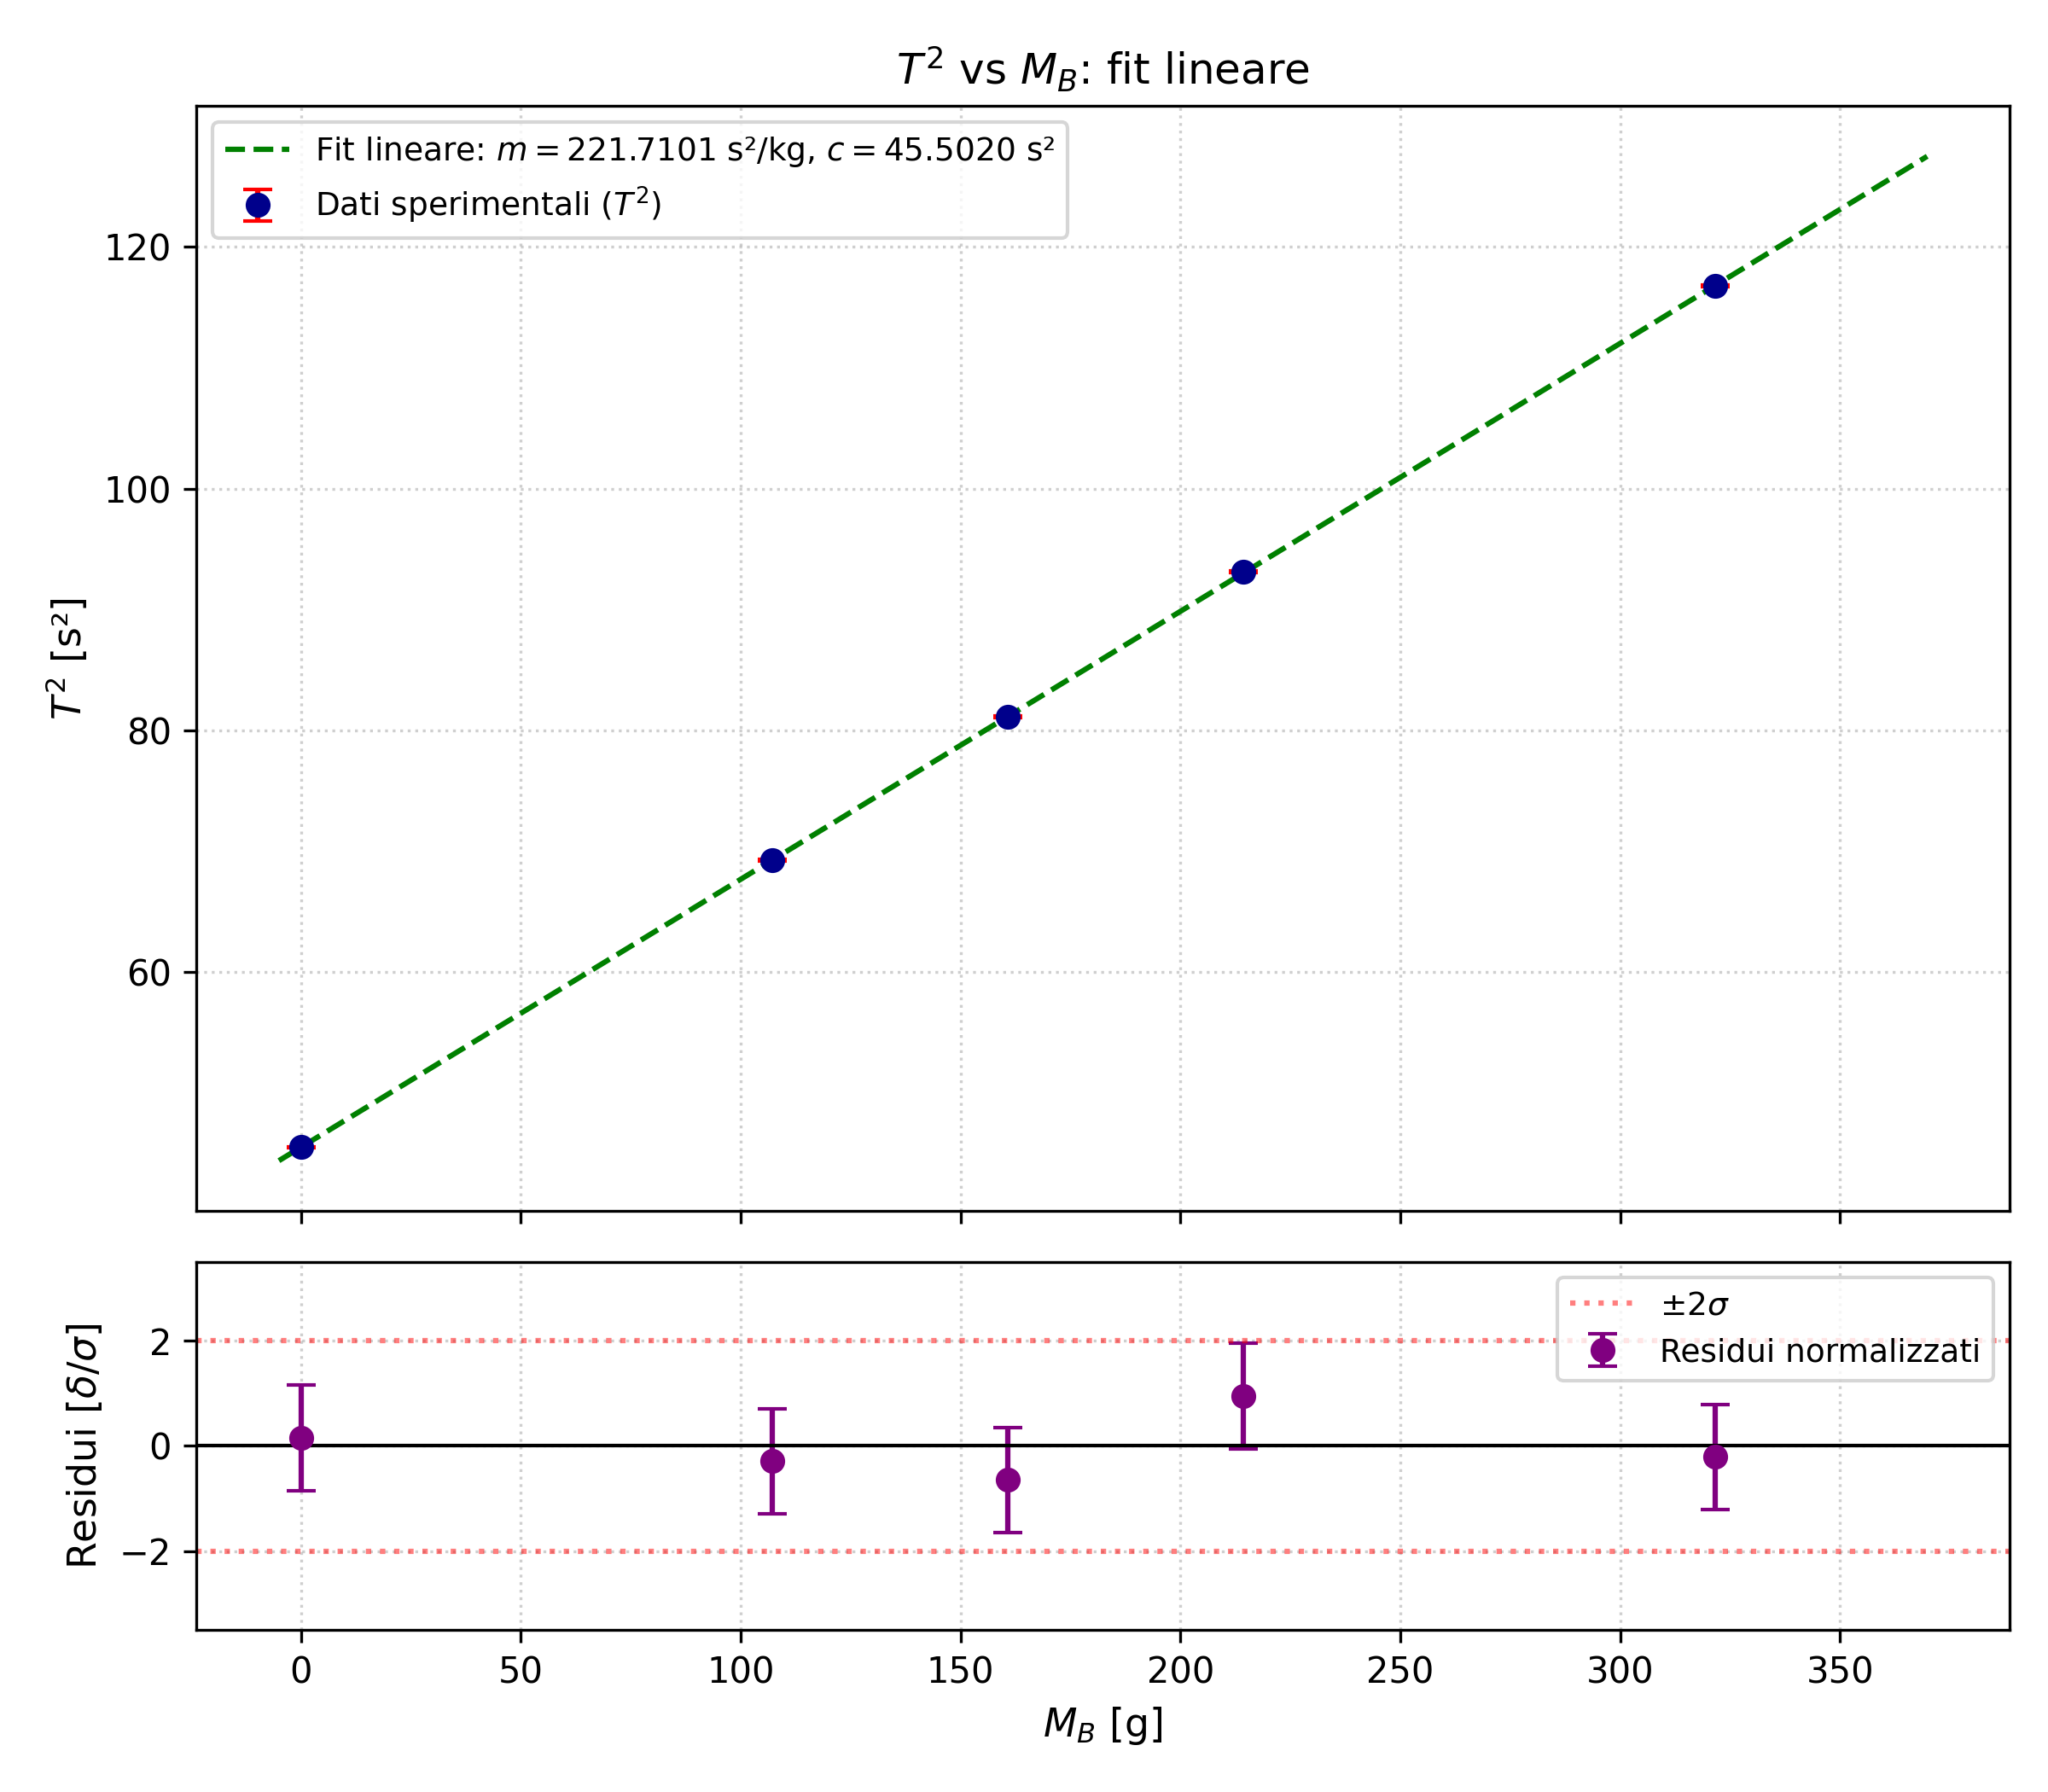
\includegraphics[scale=0.7]{fitLineare.png}
\caption{Grafico di $T^2$ vs $M_B$ con barre di errore sulle ordinate, label e unit\`a degli assi, fit lineare sovrapposto e pannello dei residui normalizzati.}
\label{fig1}
\end{figure*}

\noindent
Si nota che il punto a $n=4$ bulloni presenta un residuo normalizzato di circa $+1.2\sigma$,
compatibile con una fluttuazione statistica casuale ($|r_i| < 2$).
Il $\chi^2$ ridotto pari a $0.49$ indica che il modello lineare descrive bene i dati,
con incertezze leggermente sovrastimate.

\newpage


\section{Parte 2: descrizione delle misure, analisi dati (con le formule
  utilizzate) e risultati}

La configurazione a doppi dadi prevede 6 bulloni con 2 dadi ciascuno.
La massa totale $M_B^\mathrm{DD}$ è stata misurata direttamente con la bilancia
(pesata dell'intera configurazione).
Il periodo è stato misurato con la stessa procedura della Parte~1 (5 oscillazioni complete,
5 ripetizioni), ricavando $T_\mathrm{DD}$ e $T_\mathrm{DD}^2$ con le formule~\eqref{eq:formulaPeriodi} e~\eqref{eq:incT}.

Il valore atteso di $T^2$ è stato estrapolato dalla retta di fit:
\begin{equation}
    \hat{T}^2_\mathrm{DD} = m\,M_B^\mathrm{DD} + c
\end{equation}
con incertezza, propagando la correlazione tra $m$ e $c$:
\begin{equation}
    \sigma_{\hat{T}^2} = \sqrt{(M_B^\mathrm{DD})^2\,\sigma_m^2 + \sigma_c^2 + 2\,M_B^\mathrm{DD}\,\mathrm{Cov}[m,c]}
    \label{eq:sigmaEstr}
\end{equation}
La compatibilità tra valore estrapolato e misurato è verificata tramite:
\begin{equation}
    z = \frac{|T_\mathrm{DD}^2 - \hat{T}^2_\mathrm{DD}|}{\sqrt{\sigma_{T_\mathrm{DD}^2}^2 + \sigma_{\hat{T}^2}^2}}
\end{equation}

Tramite i risultati ottenuti, presenti nelle tabelle \ref{tab8} e \ref{tab9}, si verifica la linearità e l'attendibilità del modello teorico. 

{\def\arraystretch{1.7}\tabcolsep=12pt
	\begin{table}[h!]
		\begin{center}
			\begin{tabular}{|l|c|c|}
				\hline
				 --- & $ T_\mathrm{DD} $ & $ T_\mathrm{DD}^2 $  \\
				\hline
				--- & $11.3404 \pm 0.0036 s$& $128.605 \pm 0.082 s^2$  \\ 
				\hline				
			\end{tabular}
		\end{center}
		\caption{Periodo e periodo quadro misurato nella configurazione a doppi dadi}
		\label{tab8}
	\end{table}
}

{\def\arraystretch{1.7}\tabcolsep=12pt
	\begin{table}[h!]
		\begin{center}
			\begin{tabular}{|c|c|}
				\hline
				 $ \hat{T}^2_\mathrm{DD}\ [\mathrm{s}^2] $ & $ z $ \\
				\hline
				$128.422 \pm 0.068$ & 1.72  \\
				\hline
			\end{tabular}
		\end{center}
		\caption{Periodo quadro aspettato dall'estrapolazione tramite la retta di best fit e z-score}
		\label{tab9}
	\end{table}
}


\newpage

\section{Bonus: Stima teorica di $I_\text{disco}$ e verifica di compatibilità con $I_0$}
 
Il disco metallico ha $N=6$ fori cilindrici di raggio $r_b$ a distanza $R$ dal centro, che riducono il momento di inerzia rispetto a quello di un disco pieno. La stima teorica è:
\begin{equation}
    I_\text{teo} = \frac{1}{2}M_d r_d^2
    - N \left(\frac{1}{2}m_\text{foro}\,r_b^2 + m_\text{foro}\,R^2\right)
    \label{eq:Iteo}
\end{equation}
dove il termine $I_\text{foro}$ è il momento del cilindretto rimosso rispetto all'asse del disco, calcolato tramite il teorema degli assi paralleli ($\frac{1}{2}m_\text{foro}r_b^2$ è il momento proprio, $m_\text{foro}R^2$ è il termine di Steiner), e la massa di ciascun foro vale:
\begin{equation}
    m_\text{foro} = \rho_\text{Al}\,\pi\,r_b^2\,h_d
\end{equation}
con $\rho_\text{Al} = 2700\,\text{kg/m}^3$ densità tabulata dell'alluminio.
 
\subsection{Misure geometriche e massa del disco}
 
Il diametro $D_d$ del disco è stato misurato con il metro/squadra (risoluzione $1\,\text{mm}$, 5 ripetizioni); lo spessore $h_d$ con il calibro a nonio (risoluzione $0.05\,\text{mm}$, 5 ripetizioni). Il raggio dei fori $r_b = D_b/2$ è già noto dalla Parte~1. La massa $M_d$ è stata misurata con la bilancia; in alternativa si stima dalla geometria come $M_d = \rho_\text{Al}\,\pi\,(r_d^2 - N\,r_b^2)\,h_d$.
 
\subsection{Propagazione delle incertezze}
 
Le incertezze sulle grandezze intermedie si combinano in quadratura. Per $m_\text{foro}$:
\begin{equation}
    \frac{\sigma_{m_\text{foro}}}{m_\text{foro}} = \sqrt{\left(\frac{2\sigma_{r_b}}{r_b}\right)^2 + \left(\frac{\sigma_{h_d}}{h_d}\right)^2}
\end{equation}
Per $I_\text{foro}$, applicando la propagazione a~\eqref{eq:Iteo}:
\begin{equation}
    \sigma_{I_\text{foro}} = \sqrt{
        \left[\left(\tfrac{1}{2}r_b^2 + R^2\right)\sigma_{m_\text{foro}}\right]^2
        + \left(m_\text{foro}\,r_b\,\sigma_{r_b}\right)^2
        + \left(2\,m_\text{foro}\,R\,\sigma_R\right)^2
    }
\end{equation}
L'incertezza finale è:
\begin{equation}
    \sigma_{I_\text{teo}} = \sqrt{\sigma_{I_\text{pieno}}^2 + \left(N\,\sigma_{I_\text{foro}}\right)^2}
\end{equation}
 
\subsection{Confronto con $I_0$ dal fit}
 
La compatibilità è verificata tramite lo z-score~\eqref{eq:zBonus}. I risultati sono riportati in Tabella~\ref{tabBonus}.
 
\begin{equation}
    z = \frac{|I_0 - I_\text{teo}|}{\sqrt{\sigma_{I_0}^2 + \sigma_{I_\text{teo}}^2}}
    \label{eq:zBonus}
\end{equation}
 
{%
\def\arraystretch{1.5}\tabcolsep=10pt
\begin{table}[h!]
    \begin{center}
		\small
        \begin{tabular}{|l|c|c|c|}
            \hline
            & valore & incertezza & unità \\
            \hline
            $I_0$ (fit) & $2.7789 \times 10^{-3}$ & $0.0066 \times 10^{-3}$ & kg$\cdot$m$^2$ \\
            \hline
            $I_\text{pieno} = \frac{1}{2}M_d r_d^2$ & — & — & kg$\cdot$m$^2$ \\
            \hline
            $I_\text{foro}$ (singolo, Steiner incl.) & — & — & kg$\cdot$m$^2$ \\
            \hline
            $I_\text{teo} = I_\text{pieno} - 6\,I_\text{foro}$ & — & — & kg$\cdot$m$^2$ \\
            \hline
            $z$ & \multicolumn{3}{c|}{—} \\
            \hline
        \end{tabular}
    \end{center}
    \caption{Confronto tra $I_0$ dal fit e $I_\text{teo}$ corretto per i fori (valori numerici da inserire dopo l'esecuzione del codice).}
    \label{tabBonus}
\end{table}
}

\end{document}